\documentclass[11pt, a4paper, USenglish]{article} % change ``USenglish'' to ``norsk'' if applicable.

\usepackage{kyblab} % Contains all included packages. See kyblab.sty.
\usepackage{pgffor}
\usepackage{graphicx}
\usepackage{subcaption}
\addbibresource{bibliography.bib} % Makes the bibliography file available to biblatex.
\begin{document}

% Titlepage
\title{TTK4115 Helicopter lab report}
\author{Group 7\\Student no. 116436\\Student no. 116346\\Student no. 564341}
\date{\today}
\begin{titlepage}
    \maketitle
    \begin{figure}
    \centering
    
\includegraphics[width=0.5\textwidth]{figures/itk_ntnu}\\
    Department of Engineering Cybernetics
    \end{figure}
    \thispagestyle{empty}
\end{titlepage}

% Abstract
\newpage
\begin{abstract} 
%\addcontentsline{toc}{section}{Abstract} % add this if you want the abstract in the table of contents.
  This document highlights some of the principal components your report should include from the lab, and how it should be structured. Basic tips for formatting a report in \LaTeX{} can be found in a more extensive document which is based on work done by Tor Aksel Heirung for TTK4135, Andreas L. Fl{\aa}ten and Kristoffer Gryte \cite{LabReportExtensive}. 

  The main file, ``labreport.tex'', defines the structure of the document. 

When you write your own report, this section (the abstract) should contain a \emph{very} short summary of what the lab is about and what you have done.
\end{abstract}

\thispagestyle{empty} % Avoid page numbering on the abstract page.

% TOC
\newpage
\tableofcontents
\thispagestyle{empty} % Avoid page numbering on the table of contents.

% Main content
\newpage
\setcounter{page}{1}
\section{Introduction}\label{sec:Intro_new}

This lab is split in four parts; Use of monovariable control, use of multivariable control, use of a Luenberger observer, and lastly the Kalman filter. The monovariable control concerns non-optimal tuning of a PD controller, while multivariable control concerns optimal tuning of a multivariable controller called LQR. The use of a Luenberger observer concerns the implementation of an non-optimal estimator using measurements from an interial measurement unit (IMU), while the use of a Kalman filter concerns the implementation of an optimal estimator using
measurements from the IMU

All of these parts contribute to implement and test linear concepts around linear system theory. Throughout the lab the helicopter will become more advanced, and it will contain implementation of controllers and estimators, and
measurements from an inertial measurement unit. We will learn through hypotheses, test plans and experiments, which will be showcased in the report. Throughout the lab we will extend our understanding of controllers and estimators,
both in terms of them being non-optimal or optimal. Additionally the lab will make us aware of limitations and
possibilities when including observations/measurements from instruments like an inertial measurement unit.

The helicopter consists of a base on which a long arm is attached; see Fig. The helicopter
head, with two motors and propellers, is attached to one side of the arm. On the other side, a
counterweight is placed. The helicopter has three rotational joints. The helicopter arm can rotate
about the vertical axis. This will be referred to as the travel of the helicopter. The helicopter
head can move up and down with respect to the base. This rotation of the helicopter arm will be
referred to as the elevation of the helicopter. Moreover, the helicopter head can tilt with respect
to the arm, which will be referred to as the pitch of the helicopter. The joint angles for pitch, elevation, and travel
are measured using special counter circuits to read the encoders on the helicopter. The helicopter is actuated by the two motors on the helicopter head,
which are connected to the propellers. The control
signals (motor voltages) are set using a digital-to-analog converter (DAC). This signal is amplified
by a linear amplifier inside the power supply and fed to the motors. A model of the helicopter showcasing the axes and forces can bee seen in Fig 
\begin{figure}

\end{figure}


Your introduction should contain an overview of the work you were assigned, as well as a few sentences putting the work into a larger perspective. You can introduce the helicopter set-up such that it is easier to refer to specific variables later in the report. You should also give a quick description of how the report is organized.

You should of course put most of the work into doing good work in the lab and then presenting it in the report. When presenting your work in the report, both content and presentation/layout matters. Since your only way of communicating your good effort in the lab is through writing about it here, the way you write about it is essential. This means that even if you have a really good controller or an interesting experiment but describe it poorly, you will probably not be rewarded for the results. A plot showing perfect control is worth very little if it is not accompanied by a clear description of what it represents.


The helicopter lab is meant to be an arena for you to implement and test the theoretical concepts
covered in the lectures on a real physical system. You will be asked to complete a set of tasks,
each focusing on separate topics in the course. As you complete these tasks, the helicopter
will be gradually more advanced, with the implementation of controllers and estimators, and
measurements from an inertial measurement unit. To fully grasp the content of the course we
highly encourage you to experiment and be creative in your assigned lab time-slot. If you have
an idea of how to improve your system, or if you see something interesting to investigate further,
we encourage you to test it out! Remember to write about it in the report.
Throughout the lab you will be asked to experiment according to your hypotheses and testplans developed in the lab preparation assignment. The experiments should be done systematically and thorough, but not unnecessarily long. Remember that it is allowed to revise your
test-plan when you gain experience from testing the system.
At the end of the lab we want you to understand the concepts of controllers and estimators,
both in terms of them being non-optimal or optimal. Additionally be aware of limitations or
possibilities when including observations/measurements from instruments like an inertial
measurement unit.
\section{Part I - Monovariable control}
The goal of this task is to control the pitch of the helicopter with a PD-regulator, and set the poles to specific values. To set the poles a model of he helicopter is needed, which was prepared in the preparations. The model was derived by physical laws, and then linearized.

The test plan is to test the step response of the helicopter with different pole placement. To test the step response the reference is set to $0.5$ after $10$ second, and then to $0$ after 15 seconds, and the test is ended after $30$ seconds. The regulator parementers was calculated based on these poles. \autoref{tab:ld1:testplan1} shows the plan of which poles to test.

\begin{table}[h]
    \centering
    \begin{tabular}{ l|l } 
        Poles & Expected state \\ \hline
        pol(-1,-1) & Stable \\
        pol(-0.5, -2) & Over dampened \\
        pol(-0.5+j, -0.5-j) & Under dampened \\
        pol(-j, j) & Oscillations \\
        pol(1, 1) & Unstable \\
    \end{tabular}
    \caption{The different poles to test.}
    \label{tab:ld1:testplan1}
\end{table}

The points were picked to show different types of responses. The expected result is that poles in the right half-plane will result in a unstable system, where the pitch will go further and further away from the reference.

The points that are not at the real axis is expected to create som oscilations. In the test case where the poles are at the imaginary axis, standing oscilations are expected.

\subsection{Results}
\begin{figure}

    \centering
    \begin{subfigure}{0.40\textwidth}
      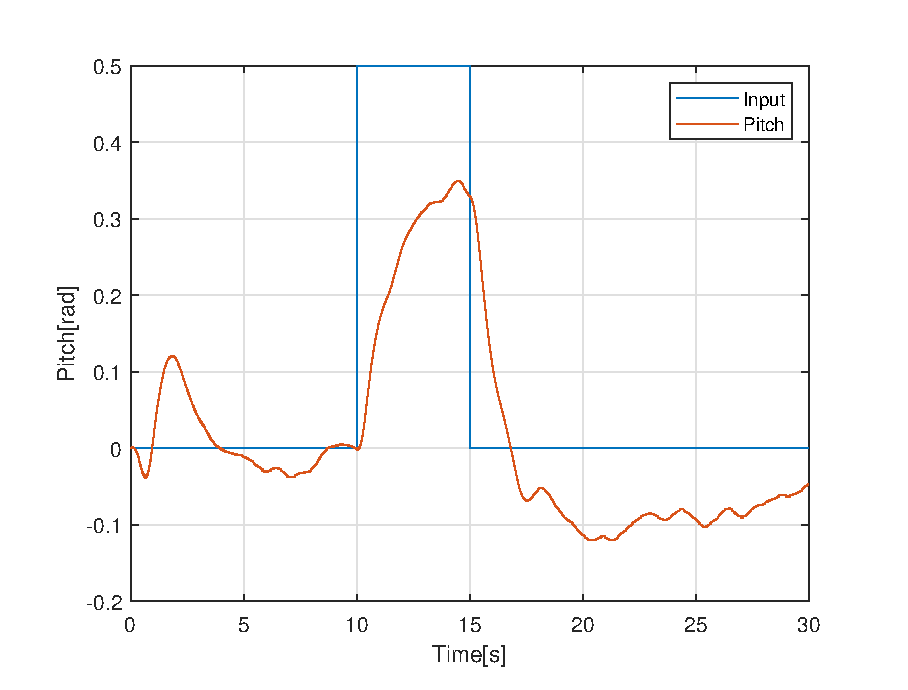
\includegraphics[width=\textwidth]{figures/labday1/-1,-1.eps}
      \caption{Poles at $-1$ and $-1$}
      \label{subfig:poles-1,-1}
    \end{subfigure}

    \begin{subfigure}{0.40\textwidth}
        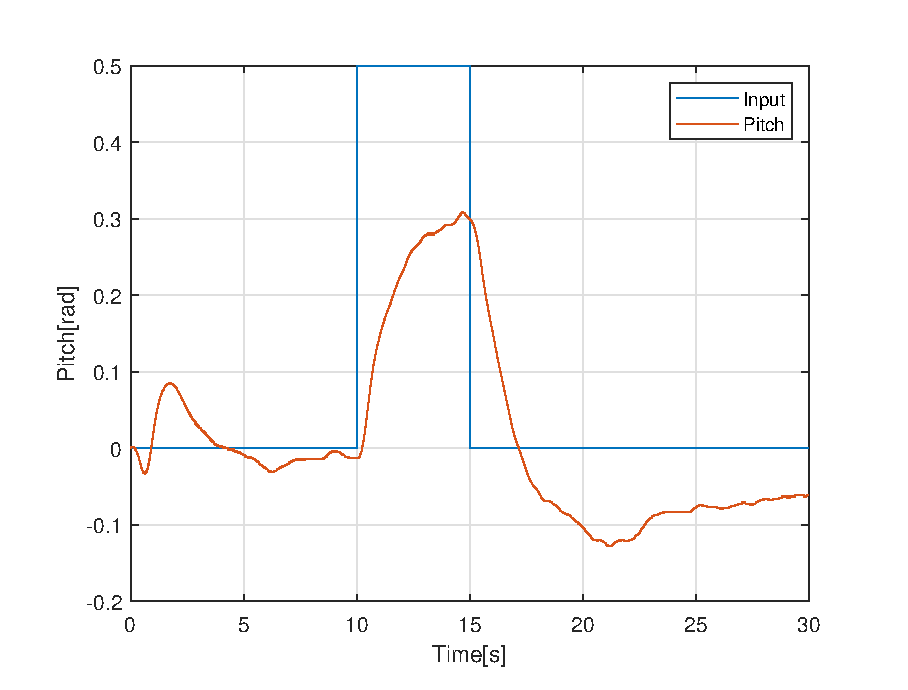
\includegraphics[width=\textwidth]{figures/labday1/-0.5,-2.eps}
        \caption{Poles at $-0.5$ and $-2$.}
        \label{fig:ld1:poles_-0.5,-2}
    \end{subfigure}
    
    \begin{subfigure}{0.40\textwidth}
        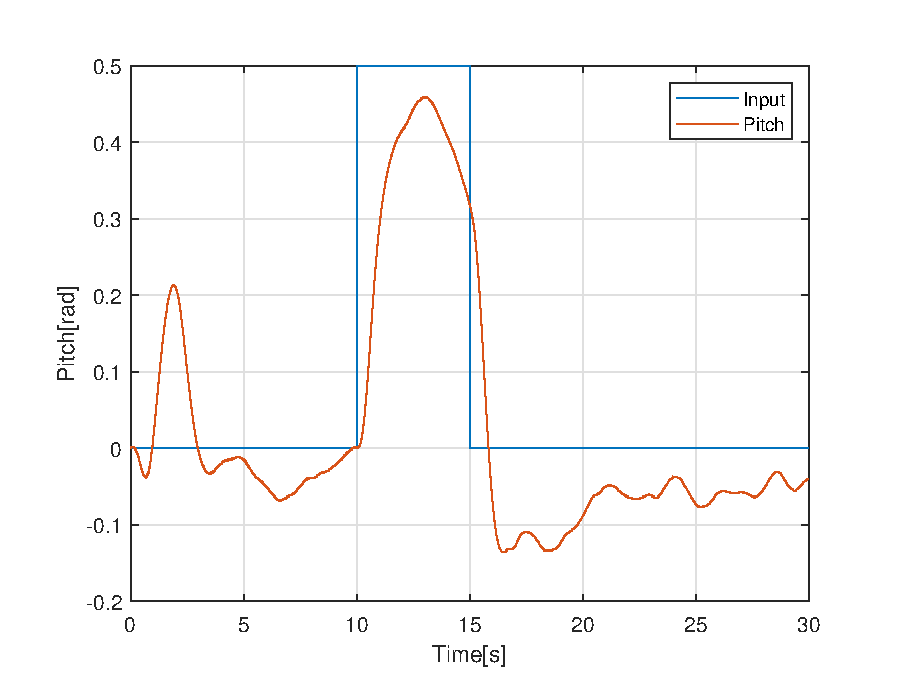
\includegraphics[width=\textwidth]{figures/labday1/-0.5+j,-0.5-j.eps}
        \caption{Poles at $-0.5+j$ and $-0.5 - j$.}
        \label{subfig:ld1:poles_-0.5+j,-0.5-j}
    \end{subfigure}

    \begin{subfigure}{0.40\textwidth}
        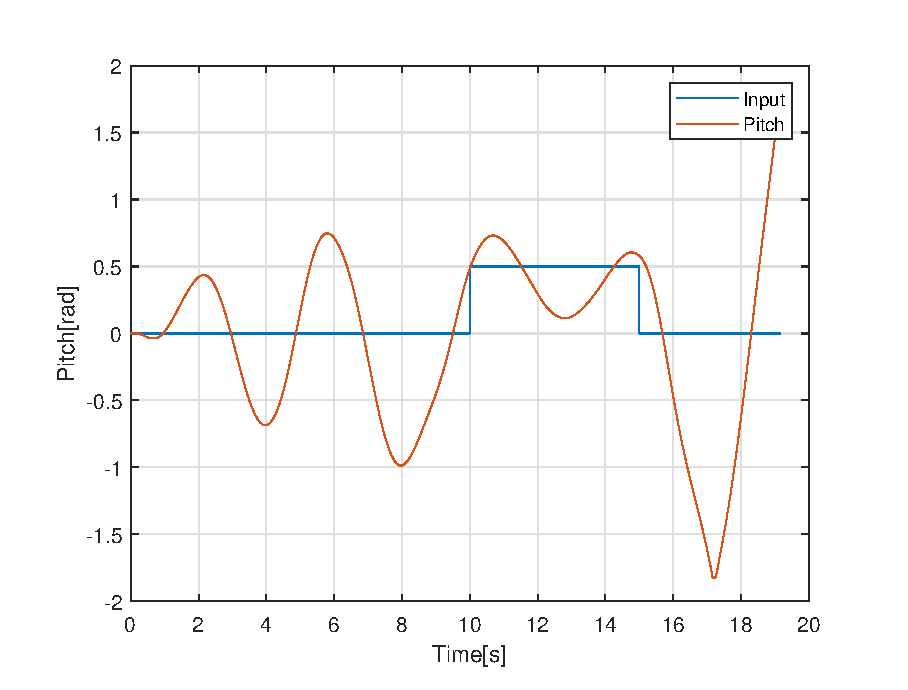
\includegraphics[width=\textwidth]{figures/labday1/j,-j.eps}
        \caption{Poles at $j$ and $-j$}
        \label{fig:ld1:poles_j,-j}   
    \end{subfigure}
        
    \begin{subfigure}{0.40\textwidth}
        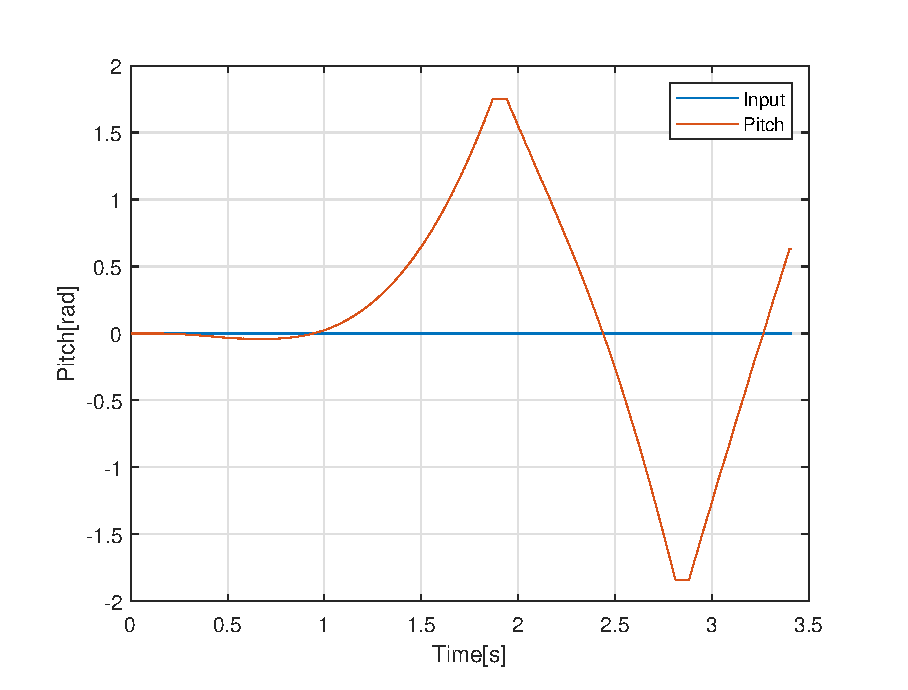
\includegraphics[width=\textwidth]{figures/labday1/1,1.eps}
        \caption{Poles at $1$ and $1$}
    \label{fig:ld1:poles_1,1}
    \end{subfigure}
    
    \caption{Results for different poles}
    \label{fig:labday1resultsdifferentpoles}
    
\end{figure}


\autoref{subfig:poles-1,-1} shows a stable response that rises quickly; however, the system never reaches the target. Indicating a stationary offset. In addition it was not expected that the pitch would go bellow $0$ after the last step function.


\autoref{subfig:ld1:poles_-0.5+j,-0.5-j} shows a response that rises faster than in \autoref{fig:ld1:poles_-1,-1}, and with minimal oscialtions. However these oscilation can be noise.


\autoref{fig:ld1:poles_-0.5,-2} show a response that more slowly reaches the reference. This can be a result of a over dampened system, which is expected with two negative poles at the real axis.



\autoref{fig:ld1:poles_j,-j} shows a response with large oscialtions. The experiment was manually stopped after the helicopter crashed. The expected response is standing oscilations, which almost matches the actual response. However the oscialtions start before the step in the reference, which can be a result of some disturbances in the system. The actual oscialtions was also increasing in amplitude a bit, which led the system to crash, therefore the experiment was stopped a bit early.



\autoref{fig:ld1:poles_1,1} show a unstable plot, where a small disturbance make the pitch increase exponentially. This lead to a fast crash and the experiment was stopped. The result was expected since the poles was in the right half-plane.

Our hypotheses were somewhat right, except that the purely imaginary poles became unstable. Also the fact that poles at $-0.5 +j$ and $0.5 + j$ gave the best response was not expected.
\section{Part II - Multivariable control}
\begin{itemize}
    \item Introduce and motivate the task. You can include a brief summary of the different tasks in the lab-preparation assignment which was necessary to complete the lab. No extensive listing or derivation of equations are needed (you can mention, e.g., LQR, controllability, integral effect, augmented matrices etc.). 
    \item Include your hypothesis/test-plan for the matrices $\mathbf{Q}_{\text{LQR}}$ and $\mathbf{R}_{\text{LQR}}$ both with and without integral effect and explain your thought process behind it. Include it if you did any experiments with the values in $\mathbf{F}$.
    \item Include the results from the experiments that were done in the lab according to the test-plan, and any other tests you found interesting during your time in the lab. Include plots and discuss the result. This is the most important part of the report. How you structure this part of the report is up to you. 
    \item Conclusion. Include a short paragraph summarizing the results.
\end{itemize}

The purpose of this task is to control the helicopter using LQR control. To do so, we first need to find the state space representation.

\begin{align*}
    \dot{x}&=Ax+Bu \\
    x&=
    \begin{bmatrix}
        p \\
        \dot{p} \\
        \dot{e} \\
    \end{bmatrix}
    \text{ and } u=
    \begin{bmatrix}
        \tilde{V_s} \\
        V_d
    \end{bmatrix}\\
    \ddot{p}&=K_1 V_d \\
    \ddot{e}&=K_2 \tilde{V_s}\\
    \dot{x}&=
    \begin{bmatrix}
        0&1&0 \\
        0&0&0 \\
        0&0&0 \\
    \end{bmatrix}
    x+
    \begin{bmatrix}
        0&0 \\
        0&K_1 \\
        K_2&0
    \end{bmatrix}
    \begin{bmatrix}
        \tilde{V_s} \\
        V_d
    \end{bmatrix}\\
\end{align*}


Then we need to make sure that 
\begin{equation*}
    \lim_{t \to \infty} \implies \dot{x} = 0 \text{ and } x = \left[
    \begin{array}{c}
        p_c \\
        0 \\
        \dot{e}_c
    \end{array}
    \right]
\end{equation*}
This gives the equation
\begin{align*}
    \dot{x} &= Ax + Bu \\
    &= (A - BK)x + BFr \\
    &= 0
\end{align*}
And solved for F we get
\begin{equation*}
    F =
    \begin{bmatrix}
        k_{11} & k_{13} \\
        k_{21} & k_{23}
    \end{bmatrix}
\end{equation*}

Such that
\begin{equation*}
    \lim_{t \to \infty} 
    \begin{bmatrix}
        p \\
        \dot{e}
    \end{bmatrix}
    =
    \begin{bmatrix}
        p_c \\
        \dot{e_c}
    \end{bmatrix}
\end{equation*}

\subsection{Hypotheses and test plan}
A high q/r will give a fast response, but with a high energy drainage. Can expect some overswing as that is a waste of energy. A low q/r will give a slow response where you minimize the amount of energy spent. We also think that high isolated Q values regulates that parameter better, at the cost of the others. We also think that implemented integral action will remove standard deviaton from the system.

This is our overarching test plan:
\begin{itemize}
    \item Try 10 on all diagonals
    \item try high q
    \item try high r
    \item try different values inside of q and r
\end{itemize}
The specific test plan for the 3-state system is shown in \autoref{tab:3stateHyp}, and the 5-state is shown in \autoref{tab:5stateHyp}.
\begin{table}[htbp]
    \centering
    \caption{Test values for 3 state LQR}
    \begin{tabular}{c|ccccc}
        \textbf{Test} & \( Q_p \) & \( Q_{\dot{p}} \) & \( Q_{\dot{e}} \) & \( R_{\tilde{V}_s} \) & \( R_{V_d} \) \\
        \hline
        1  & 10  & 10  & 10  & 10  & 10  \\
        2  & 200 & 10  & 10  & 10  & 10  \\
        3  & 10  & 200 & 10  & 10  & 10  \\
        4  & 10  & 10  & 200 & 10  & 10  \\
        5  & 10  & 10  & 10  & 200 & 10  \\
        6  & 10  & 10  & 10  & 10  & 200 \\
        7  & 200 & 200 & 200 & 10  & 10  \\
        8 & 10  & 10  & 10  & 200 & 200 \\
    \end{tabular}
    \label{tab:3stateHyp}
\end{table}

\begin{table}[htbp]
    \centering
    \caption{Test values for 5 state LQR}
    \begin{tabular}{c|ccccccc}
        \textbf{Test} & \( Q_p \) & \( Q_{\dot{p}} \) & \( Q_{\dot{e}} \) & \( Q_{\dot{\gamma}} \) & \( Q_{\dot{\zeta}} \) & \( R_{\tilde{V}_s} \) & \( R_{V_d} \) \\
        \hline
        1  & 10  & 10  & 10  & 10  & 10  & 10  & 10  \\
        2  & 200 & 10  & 10  & 10  & 10  & 10  & 10  \\
        3  & 10  & 200 & 10  & 10  & 10  & 10  & 10  \\
        4  & 10  & 10  & 200 & 10  & 10  & 10  & 10  \\
        5  & 10  & 10  & 10  & 200 & 10  & 10  & 10  \\
        6  & 10  & 10  & 10  & 10  & 200 & 10  & 10  \\
        7  & 10  & 10  & 10  & 10  & 10  & 200 & 10  \\
        8  & 10  & 10  & 10  & 10  & 10  & 10  & 200 \\
        9  & 200 & 200 & 200 & 200 & 200 & 10  & 10  \\
        10 & 10  & 10  & 10  & 10  & 10  & 200 & 200 \\
    \end{tabular}
    \label{tab:5stateHyp}
\end{table}
% Helper function to plot subfigures fast
% #1 = path prefix, #2 = number of figures
\newcommand{\insertsubfigs}[2]{%
  \foreach \i in {1,...,#2}{%
    \begin{subfigure}{0.40\textwidth}
      \includegraphics[width=\textwidth]{#1\i.eps}
      \caption{Results for test \i.}
    \end{subfigure}
  }%
}

\subsection{Results}
From \autoref{fig:LQR_3state}, we see that there is a lot of standard deviation in the 3 state system. We see overall better results, without standard deviation, for the 5-state regulator (\autoref{fig:LQR_5state}), as expected. In the 5-state system, the results from test 2 in \autoref{fig:LQR_5state}. were the best, which makes sense since we tested pitch, and the cost of bad pitch was proportionally higher than everything else in test 2. We also see that test 9 was better than a lot of the others with high Q, which confirmes that to increase the cost of one state, affects the other states. For instance test 3 was quite bad for the pitch.

\begin{figure}[h!]
    \centering
    \insertsubfigs{figures/labday2/3state/plot_}{8}
    \caption{Step response for the three-state LQR regulator.}
    \label{fig:LQR_3state}
\end{figure}



\begin{figure}[h]
    \centering
    \insertsubfigs{figures/labday2/5state/plot_}{10}
    \caption{Step response for the five-state LQR regulator.}
    \label{fig:LQR_5state}
\end{figure}
\section{Part III - Luenberger observer}
\begin{itemize}
    \item Introduce and motivate the task. You can include a brief summary of the different tasks in the lab-preparation assignment which was necessary to complete the lab. No extensive listing or derivation of equations are needed (you can mention, e.g., the IMU, noisy measurements, observability, state-estimation etc.).
    \item Did you find out the minimum set of states that if measured makes the system observable? Did you experiment with this?
    \item Include your hypothesis/test-plan for the estimator poles and explain your thought process behind it.
    \item Include the results from the experiments that were done in the lab according to the test-plan, and any other tests you found interesting during your time in the lab. Include plots and discuss the result. This is the most important part of the report. How you structure this part of the report is up to you. 
    \item Conclusion. Include a short paragraph summarizing the results. 
\end{itemize}

Given the system
\begin{equation*}
    \begin{bmatrix}
        \dot{p} \\
        \ddot{p} \\
        \dot{e} \\
        \ddot{e} \\
        \ddot{\lambda}
    \end{bmatrix}
    &=
    \begin{bmatrix}
        0 & 1 & 0 & 0 & 0 \\
        0 & 0 & 0 & 0 & 0 \\
        0 & 0 & 0 & 1 & 0 \\
        0 & 0 & 0 & 0 & 0 \\
        K_3 & 0 & 0 & 0 & 0
    \end{bmatrix}
    \begin{bmatrix}
        p \\
        \dot{p} \\
        e \\
        \dot{e} \\
        \dot{\lambda}
    \end{bmatrix}
    +
    \begin{bmatrix}
        0 & 0 \\
        0 & K_1 \\
        0 & 0 \\
        K_2 & 0 \\
        0 & 0
    \end{bmatrix}
    \begin{bmatrix}
        \tilde{V_s} \\
        V_d
    \end{bmatrix}
\end{equation*}

We need to measure ($p$ or $\dot{p}$) and ($e$ or $\dot{e}$) and $\lambda$ to be observe the whole system. We need to measure all these states since they are disconnected systems, and therefore need different measurements.



\section{Part IV - Kalman filter}
\begin{itemize}
    \item Introduce and motivate the task. You can include a brief summary of the different tasks in the lab-preparation assignment which was necessary to complete the lab. No extensive listing or derivation of equations are needed (you can mention, e.g., measurement noise, process noise, optimal estimator, etc.). 
    \item Include your hypothesis/test-plan and explain your thought process behind it.
    \item Include the results from the experiments that were done in the lab according to the test-plan, and any other tests you found interesting during your time in the lab (bonus tasks?). Include plots and discuss the result. This is the most important part of the report. How you structure this part of the report is up to you. 
    \item Conclusion. Include a short paragraph summarizing the results. 
\end{itemize}

The goal of this task is to implement and tune a Kalman filter, such that we get a stable system.
The matrices for the 6-state system looks like this:
\begin{equation}
    \begin{aligned}
        \mathbf{A}&=
        \begin{bmatrix}
            0 & 1 & 0 & 0 & 0 &0 \\
            0 & 0 & 0 & 0 & 0 & 0\\
            0 & 0 & 0 & 1 & 0 & 0\\
            0 & 0 & 0 & 0 & 0 & 0\\
            0 & 0 & 0 & 0 & 0 & 1\\
            K_3 & 0 & 0 & 0 & 0 & 0
        \end{bmatrix}\\
        \mathbf{B}&=
        \begin{bmatrix}
            0 & 0 \\
            0 & K_1 \\
            0 & 0 \\
            K_2 & 0 \\
            0 & 0 \\
            0 & 0
        \end{bmatrix}\\
        \mathbf{C}&=
        \begin{bmatrix}
            1 & 0 & 0 & 0 & 0 & 0 \\
            0 & 1 & 0 & 0 & 0 & 0\\
            0 & 0 & 1 & 0 & 0 & 0\\
            0 & 0 & 0 & 1 & 0 & 0\\
            0 & 0 & 0 & 0 & 0 & 1
        \end{bmatrix}\\
    \end{aligned}
\end{equation}

The discrete-time system is given with these matrices
\begin{equation}
    \mathbf{A_d}=\mathbf{A}\cdot t +\mathbf{I},\
    \mathbf{B_d}=\mathbf{B}\cdot t,\
    \mathbf{C_d}=\mathbf{C}
\end{equation}
\subsection{Hypothesis and test plan}
We will implement the kalmanfilter in simulink, and try out different values along the diagonal of $Q_d$. The test plan is shown in \autoref{tab:Kalmantestplan}. We will also apply external disturbances to test how the system handles that.

\begin{table}[htbp]
    \centering
    \caption{Test diagonal values in $Q_d$}
    \begin{tabular}{c|ccccc}
        \textbf{Test} & $Q_1$ & $Q_2$ & $Q_3$ & $Q_4$ & $Q_5$ \\
        \hline
        1 &0  & 0  & 0  & 0  & 0  \\
        2 &1000  & 1000  & 1000  & 1000  & 1000  \\
        3 &1  & 1  & 1  & 1  & 1  \\
    \end{tabular}
    \label{tab:Kalmantestplan}
\end{table}
Our hypothesis is that when all q values are 0, the filter will only follow the model. We also think that when all Q values are 1000, the filter will only follow the measurements. With all Q values set to 1, we believe we will obtain something in between, hopefully not too noisy.

\subsection{Results}
Our hypothesis was somewhat right. The edge cases of 0 and 1000 was right, but with Q values along 1, the estimated states were still wery noisy. Therefore we first tuned all diagonal values in Q toghether until we were somewhat satisfied with $\hat{x}$. This happend with $10^{-5}$. After that we tuned the different states seperately, and ended up with the $Q_d$ matrix shown in \autoref{eq:kalmanqmatrix}. Since we have no measurement of $\lambda$, we sat that value to 0.
\begin{equation}
    \begin{aligned}
        \mathbf{Q_d}&=
        \begin{bmatrix}
            10^{-6} & 0 & 0 & 0 & 0 & 0 \\
            0 & 10^{-5} & 0 & 0 & 0 & 0\\
            0 & 0 & 10^{-6} & 0 & 0 & 0\\
            0 & 0 & 0 & 10^{-5} & 0 & 0\\
            0 & 0 & 0 & 0 & 0 & 0\\
            0 & 0 & 0 & 0 & 0 & 10^{-4}
        \end{bmatrix}\\
    \end{aligned}
    \label{eq:kalmanqmatrix}
\end{equation}

In \autoref{fig:plotavkalman}, you can see the the different states in $\hat{x}$ compared to the IMU output while applying a lot of external disturbance. The kalman filter handles both IMU noise and external disturbances well.

\begin{figure}

    \centering
    \begin{subfigure}{0.40\textwidth}
      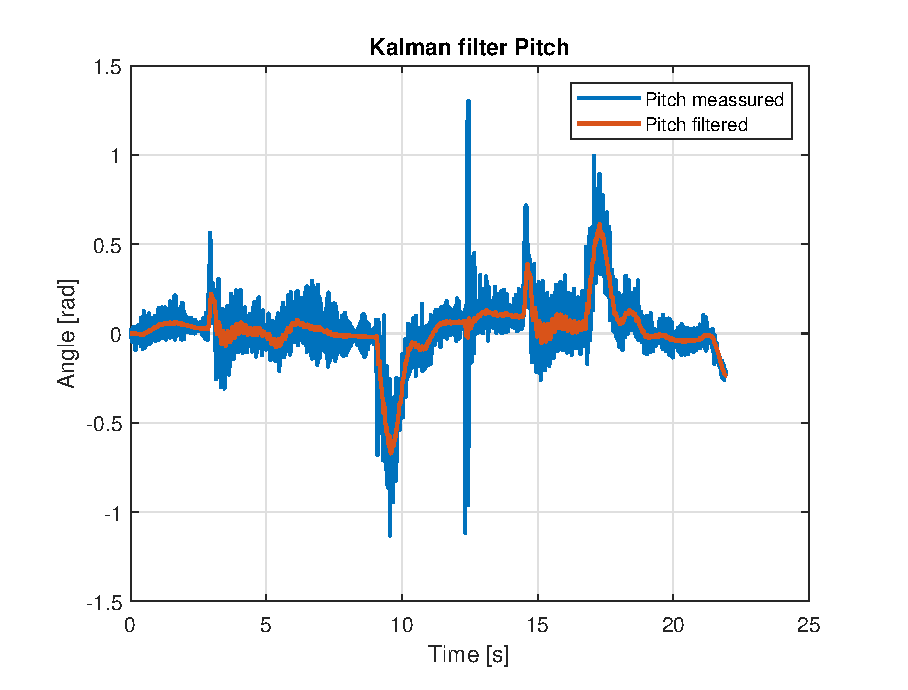
\includegraphics[width=\textwidth]{figures/labday4/p.eps}
      \caption{$p$}
    \end{subfigure}

    \begin{subfigure}{0.40\textwidth}
        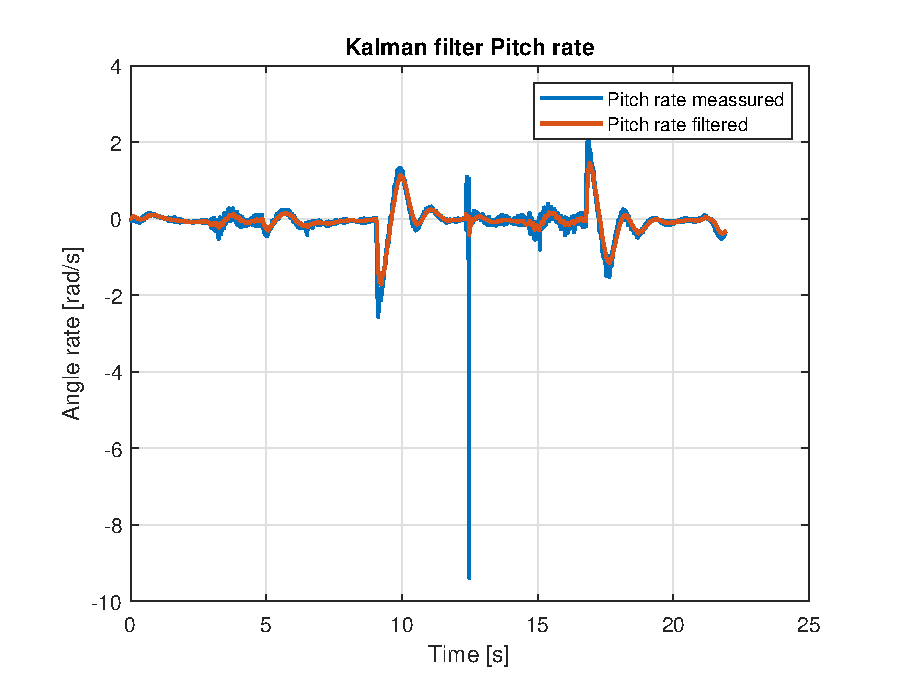
\includegraphics[width=\textwidth]{figures/labday4/p_dot.eps}
        \caption{$\dot{p}$}
    \end{subfigure}
    
    \begin{subfigure}{0.40\textwidth}
        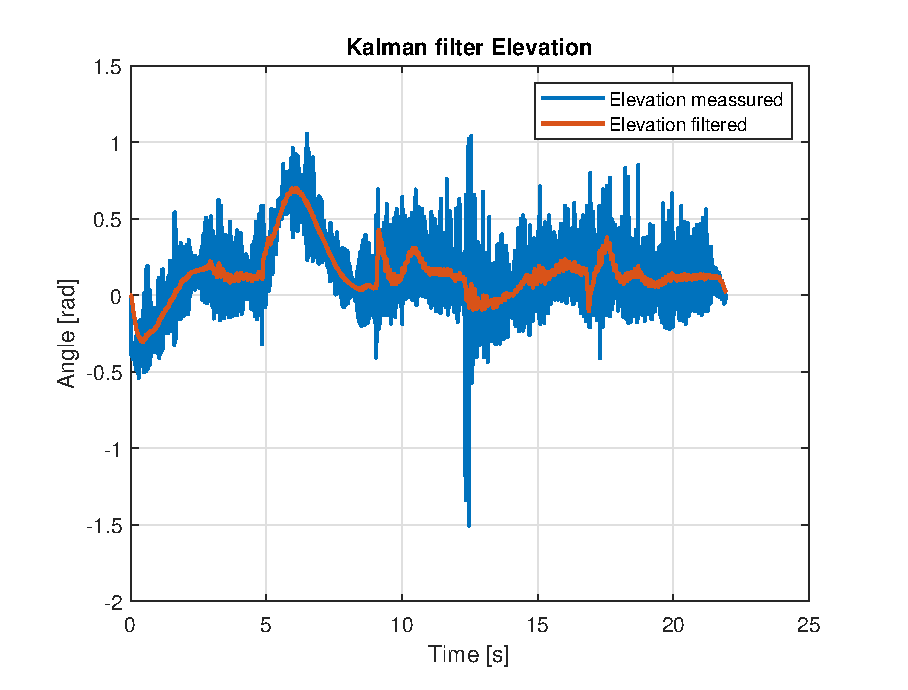
\includegraphics[width=\textwidth]{figures/labday4/e.eps}
        \caption{$e$}
    \end{subfigure}

    \begin{subfigure}{0.40\textwidth}
        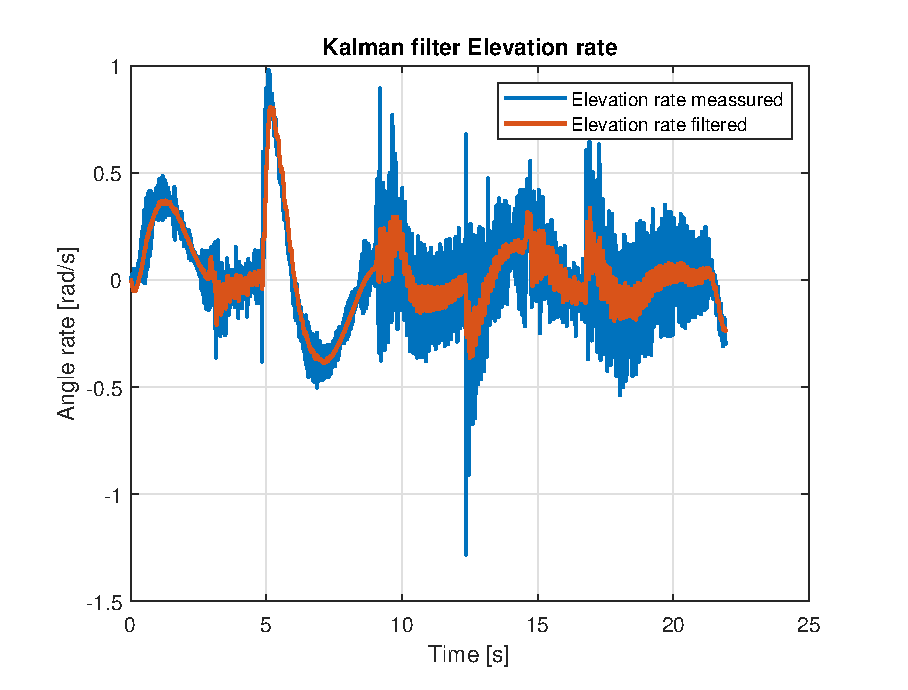
\includegraphics[width=\textwidth]{figures/labday4/e_dot.eps}
        \caption{$\dot{e}$}   
    \end{subfigure}
        
    \begin{subfigure}{0.40\textwidth}
        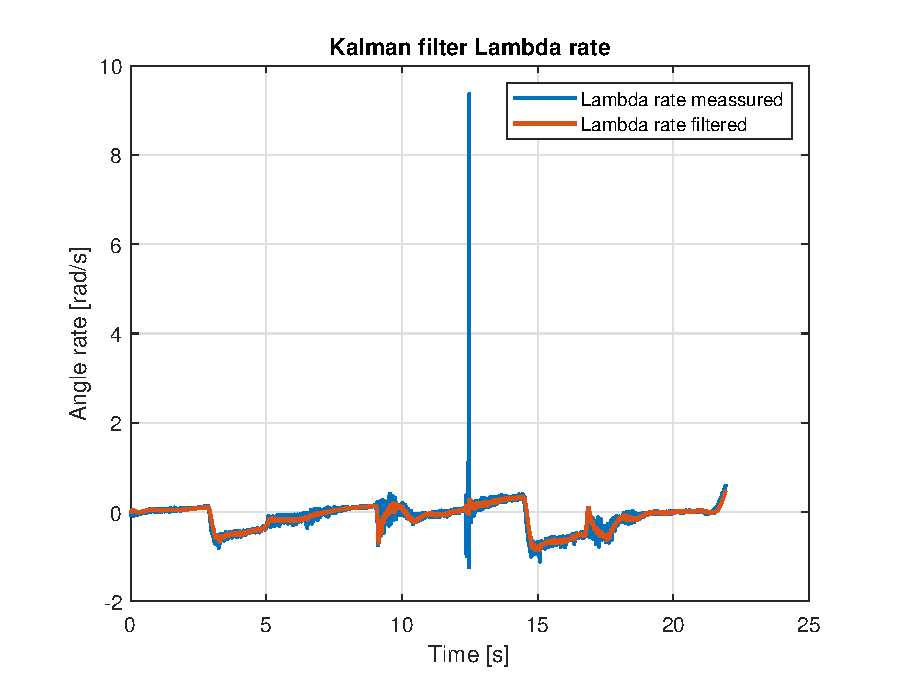
\includegraphics[width=\textwidth]{figures/labday4/lambda_dot.eps}
        \caption{$\dot{\lambda}$}
    \end{subfigure}
    
    \caption{Results for different poles}
    \label{fig:plotavkalman}
    
\end{figure}

% \input simply inserts the contents of the file, while \include forces a \newpage.
% See \input vs. \include: http://tex.stackexchange.com/questions/246/when-should-i-use-input-vs-include

% References
\newpage
\addcontentsline{toc}{section}{References}
\printbibliography{}
\label{sec:bibliography}

\end{document}
